\chapter{Analyse}\label{ch:analyse}
Im Folgendem erfolgt eine Beschreibung der Beispielanwendung \glqq DATEV-Rechnungsschreibung\grqq.
Die dafür benötigten Informationen stammen aus Gesprächen mit Mitarbeiter 1 aus der Abteilung, die für die DATEV-Rechnungsschreibung zuständig ist.
Es wird vor allem der technische Aspekt beleuchtet.
Anschließend wird der aktuelle Bereitstellungsprozess für die Laufzeitumgebung, dem dazugehörigen Datenbanksystem und einer Messaging Lösung dargestellt.

\section{DATEV-Rechnungsschreibung}
Für diese Arbeit wurde die DATEV-Rechnungsschreibung als Beispielanwendung herangezogen, weil sie folgenden Anforderungen entspricht.
Es handelt sich zum einem um eine in sich abgeschlossene Anwendung, die nur zu Beginn des Prozesses von anderen Anwendungen abhängig ist.
Zum anderen benötigt die DATEV-Rechnungsschreibung ein CICS als Laufzeitumgebung, eine Db2-Datenbank und IBM MQ als Messaginglösung.
Somit kann ein umfangreicher Bereitstellungsmechanismus in dieser Arbeit untersucht werden.

\subsection{Beschreibung}\label{rechBesch}
Bei dem Gesamtablauf handelt es sich um einen Batch-Ablauf auf dem Großrechner der DATEV e.G.
Ein wesentlicher Teil der Preisermittlung ist aus Grund einer besseren Performance als CICS-Anwendung implementiert.
Zunächst wird nach jeder kostenpflichtigen Leistungserbringung durch die dazugehörige Anwendung ein Berechnungssatz erzeugt.
Ein Berechnungssatz beinhaltet die Metainformationen der Berechnung unter anderem die Artikelnummer, Menge und den Kundenbegriff.
Preis und die Kundenzuordnung werden zu einem späteren Zeitpunkt innerhalb der DATEV-Rechnungsschreibung ermittelt.

\subsubsection{Einpflegung Berechnungssätze}
Für das Einpflegen der Berechnungssätze in den DATEV Rechnungsschreibungsablauf stehen den Anwendungen drei Möglichkeiten zur Verfügung.
\begin{itemize}
\item DMVINF-Schnittstelle
\item Webservice-Schnittstelle
\item CSV-Datei
\end{itemize}

Bei der Ersten Möglichkeit handelt es sich um die Verwendung der DMVINF\footnote{DatevMakroVerarbeitungsinformation}-Schnittstelle.
Die Schnittstelle ist in der Programmiersprache Assembler entwickelt.
Somit ist diese nur auf dem Mainframe verfügbar.
Das Ergebnis der Schnittstelle ist eine sequentielle Datei am Großrechner, vergleichbar mit einer .txt Datei unter Windows.
Diese Datei, auch Berechnungsdatei genannt, hat folgenden Aufbau.
Der erste Satz enthält Steuerinformationen, wie zum Beispiel Datum/Uhrzeit, Produkt usw.
Danach kommen die eigentlichen Berechnungssätze.
Schließlich folgt noch die Anzahl der Sätze und die Summe der einzelnen Artikel in einem Satz mit Kontrollinformationen.
Diese Kontrollinformationen werden im weiteren Verlauf mit den eingelesenen Werten abgeglichen, dadurch werden Fehler und mutwillige Änderungen der Daten von außen ausgeschlossen.
Aus dem Aufbau einer solchen Datei lässt sich schließen, dass verschiedene Schritte für die Erzeugung innerhalb der Anwendung notwendig sind.

Für die nachfolgenden Schritte stellt die DMVINF-Schnittstelle jeweils Funktionen zur Verfügung.
Zuerst wird beim sogenannten \glqq Open\grqq{} die Datei erstellt und der Steuersatz geschrieben.
Danach folgt das eigentliche Schreiben der Berechnungssätze, dabei dürfen nur bestimmte Felder (Kundenbegriffe und Mengen) verändert werden.
Unzulässige Änderungen haben einen Abbruch des Ablaufs zur Folge.
Schließlich folgt noch der \glqq Close\grqq{} bei dem die Kontrollinformationen geschrieben werden.
Hinzuzufügen ist, dass die variablen Informationen einer Formalprüfung unterzogen werden.
So entstehen je nach fachlicher Logik und Laufhäufigkeit der Anwendung mehrere Berechnungsdateien.

Eine weitere Möglichkeit, die Berechnungsinformationen in den Ablauf einzupflegen ist, die Übergabe durch einen in der Programmiersprache Java realisierten SOAP-WebService.
Hier werden die Berechnungsinformationen in XML-Format bereitgestellt.
Dadurch ist eine plattformübergreifende Weitergabe der Daten möglich.
Das Ergebnis der entsprechenden Plausibilitätsprüfungen, die in einem Onlineverfahren durchgeführt werden, wird direkt an die aufrufende Anwendung zurückgegeben.
Sind die Daten korrekt werden diese vorerst in einer Datenbank gespeichert.
Vor dem nächsten Schritt wird diese Datenbank ausgelesen und mit der ersten Möglichkeit in den Kernablauf eingespeist.

Bei der letzten Möglichkeit handelt es sich um die Übergabe mittels einer CSV-Datei.
Die Datei wird auf den Großrechner übertragen und dort mit der DMVINF-Schnittstelle verarbeitet.
Dieses Verfahren wird kaum von produktiven Anwendungen sondern hauptsächlich für Test- oder Qualitätssicherungszwecke genutzt.

Mittels dieser drei Möglichkeiten werden insgesamt monatlich circa 30 Millionen Datensätze bereitgestellt und weiterverarbeitet.
Diese Datensätze stehen innerhalb der durch die DMVINF-Schnittstelle, den Webservice oder die CSV-Datei erzeugten Berechnungsdateien dem weiteren Verlauf als Input zur Verfügung.
Um sicherzustellen, dass all diese Dateien auch verarbeitet werden, wird bei Erstellung einer solchen Berechnungsdatei ein Eintrag in eine Kontrolldatei vorgenommen.
In dieser Kontrolldatei wird jedes Lesen und somit auch das Lesen im weiteren Verlauf gekennzeichnet.
Eine monatliche Überprüfung führt die zuständige Abteilung manuell durch. 

\subsubsection{Tägliche Bewertung}\label{sssec:täglbew}
Der nächste Schritt des DATEV Rechnungsschreibungsprozesses ist die sogenannte \glqq Tägliche Bewertung\grqq.
Dieser Ablauf läuft einmal täglich von Montag bis Freitag und ist für die Preisermittlung und Kundenzuordnung zuständig.
Zur Realisierung wurden die Programmiersprachen Assembler, COBOL und Java genutzt.
Am Ende dieses Ablaufes steht die ARUBA\footnote{Abrechnungs- und Umsatz-Basis}-Db2-Datenbank.
Dort werden die Berechnungsdaten der letzten 36 Monate aufbewahrt.
Dabei handelt es ich um insgesamt circa 3,8 Milliarden Datensätze von einer Gesamtgröße von circa 400 GB mit Indizes.
Diese Datensätze beinhalten alle Informationen für die endgültige Erzeugung der Rechnungen.

Der erste Schritt der Täglichen Bewertung ist das Zusammenführen der Berechnungsdateien aus dem vorherigen Schritt und aus den bereits vorhandenen Daten des laufenden Monats aus der ARUBA-Db2-Datenbank.
Zusätzlich werden während dieser Zusammenführung den Berechnungssätzen auf Basis der abgebenden Anwendung die entsprechenden Rechnungsstellungsrhythmen (täglich oder monatlich) zugewiesen.
Anschließend wird mit Hilfe der Beraternummer die zugehörigen Betriebsstätte-, Rechnungsempfänger-, Hauptberater- und Mitglieds- bzw. Geschäftspartnernummer ermittelt.
Die Beraternummer ist als oberster Kundenbegriff in den Berechnungssätzen enthalten.
Außerdem wird die Debitorenkontonummer entweder durch die Mitglieds- oder durch die Geschäftspartnernummer zugeordnet.
Für die Preisermittlung werden die Datensätze nach Geschäftspartner gruppiert.
Im DATEV e.G. Umfeld ist ein Geschäftspartner entweder eine Kanzlei oder ein einzelner Mandant.

Dann werden die gruppierten Daten in eine CICS-Anwendung übertragen. Die Entscheidung, die Anwendung in CICS zu hosten hatte die zuständige Abteilung aus Performancegründen getroffen.
Die Architektur der CICS-Anwendung wird in \ref{rechArch} beschrieben.
Dort findet die Preisermittlung mit den dazugehörigen kundenindividuellen Abhängigkeiten, wie zum Beispiel Rabatten, statt.
Anschließend werden die Daten wieder zurück an den Batch-Ablauf übertragen.
Hier werden die Rechnungsnettobeträge geprüft, z.B. ob diese über einem bestimmten Rechnungslimitbetrag liegen.
Wird dieser Rechnungslimitbetrag unterschritten werden die Berechnungssätze als BUL\footnote{Berater unter Limit} gekennzeichnet und in die folgende Rechnungsperiode vorgetragen.
Schließlich wird noch die Umsatzsteuer ermittelt.
Abschließend werden die neu erzeugten Berechnungsdaten in die ARUBA-Db2-Datenbank eingepflegt und entsprechend gekennzeichnet.

\subsubsection{Rechnungsaufbereitung}
Als letzter Schritt folgt die Rechnungsaufbereitung.
Diese erfolgt am ersten Werktag im Monat.
Mit Hilfe der ARUBA-Db2-Datenbank wird ermittelt, welchen Kunden eine Rechnung zugestellt werden muss.
Außerdem wird dabei der Zustellungsweg, beispielsweise Post oder E-Mail, bestimmt.
Darauf folgt die Aufbereitung der Druckrohdaten und letztlich das Versenden der Rechnungen an die Berater.
Zusätzlich werden die Rechnungen noch im PDF-Format archiviert.

\subsection{Architektur der Preisermittlung}\label{ssec:recharch}
In dieser Arbeit steht das automatisierte Provisionieren von Laufzeitumgebungen im Fokus.
In diesem Fall handelt es sich um die Laufzeitumgebung CICS mit den dazugehörigen Elementen.
Im Folgenden wird nur auf den Aufbau dieser Umgebung und dessen Gründe eingegangen.

Das System muss an Lasttagen bis zu 180.000 Geschäftspartner verarbeiten können.
Die Verarbeitung eines Geschäftspartners wird von einer Transaktion durchgeführt.
So sind an Lasttagen 180.000 Transaktionen vom System zu verarbeiten.
Um all diese an das CICS zu übertragen, stehen dem System mehrere IBM MQ Queues zur Verfügung.
Bevor die eigentliche Ermittlung der Preise stattfindet, werden zunächst die Preisinformationen und die kundenindividuellen Preisabhängigkeiten, wie zum Beispiel Rabatte, ermittelt.
Für die Verarbeitung werden zwei weitere Queues verwendet.
Eine startet eine Transaktion im CICS, die andere wartet auf deren Antwort.
Innerhalb der Transaktion werden alle benötigten Preisinformationen und -abhängigkeiten mit Hilfe einer Db2 Datenbank ermittelt.
Diese Informationen werden dann in einem sogenannten \glqq SHARED GETMAIN\grqq-Bereich gespeichert.
Dabei handelt es sich im Prinzip um einen Hauptspeicherbereich, der dem CICS zur Verfügung steht.
Die Adresse dieses Bereiches wird den Transaktionen zur Verfügung gestellt.
Somit greifen die einzelnen Transaktionen nicht mehr direkt auf die Datenbank zu, sondern stattdessen auf den schnelleren Hauptspeicher.
Diese Vorarbeit ist notwendig, da es aufgrund von bis zu 60 Millionen Datenbankzugriffen zu massiven Einbußen bezüglich der Performance führen würde.

Die Queues, die für die Bestimmung der Preise benötigt werden, werden im Folgenden beschrieben.
Darunter ist eine allgemeine Queue in der alle Aufträge, die für die Weiterverarbeitung zur Verfügung stehen, geschrieben werden.
Pro Geschäftspartner wird ein Auftrag angelegt.
In diesem Auftrag befinden sich die Namen vier weiterer Queues.
Eine dieser Queues beinhaltet alle Informationen, die für die Preisermittlung des dazugehörigen Geschäftspartners notwendig sind.
Hierzu zählt unter anderem die Adresse des vorher beschriebenen Hauptspeicherbereichs.
In den restlichen drei Queues sind die Ergebnisse der Preisermittlung gespeichert.
Die Ergebnisse stehen somit dem Batch-Ablauf zur Weiterverarbeitung zur Verfügung.
Für jede der vier Queues existieren jeweils 100 vorgefertigte Namen.
Somit können auch maximal nur 100 Aufträge gleichzeitig auf Weiterverarbeitung warten.
Falls dieses Limit erreicht ist, wartet der Batch-Ablauf so lange, bis einer der Aufträge fertig gestellt wird.
Sobald ein Auftrag in die allgemeinen Auftragsqueue geschrieben wird, wird eine CICS-Transaktion gestartet.
Diese führt die Preisermittlung durch und schreibt das Ergebnis auf die dazugehörigen Queues.
Ist dies geschehen, stehen die Queues wieder für einen neuen Auftrag zur Verfügung.
Es können maximal 30 Transaktionen zeitgleich arbeiten.

\section{Aktueller Bereitstellungsprozess}\ref{sec:aktbereit}
 \begin{figure}[ht!]
\centering
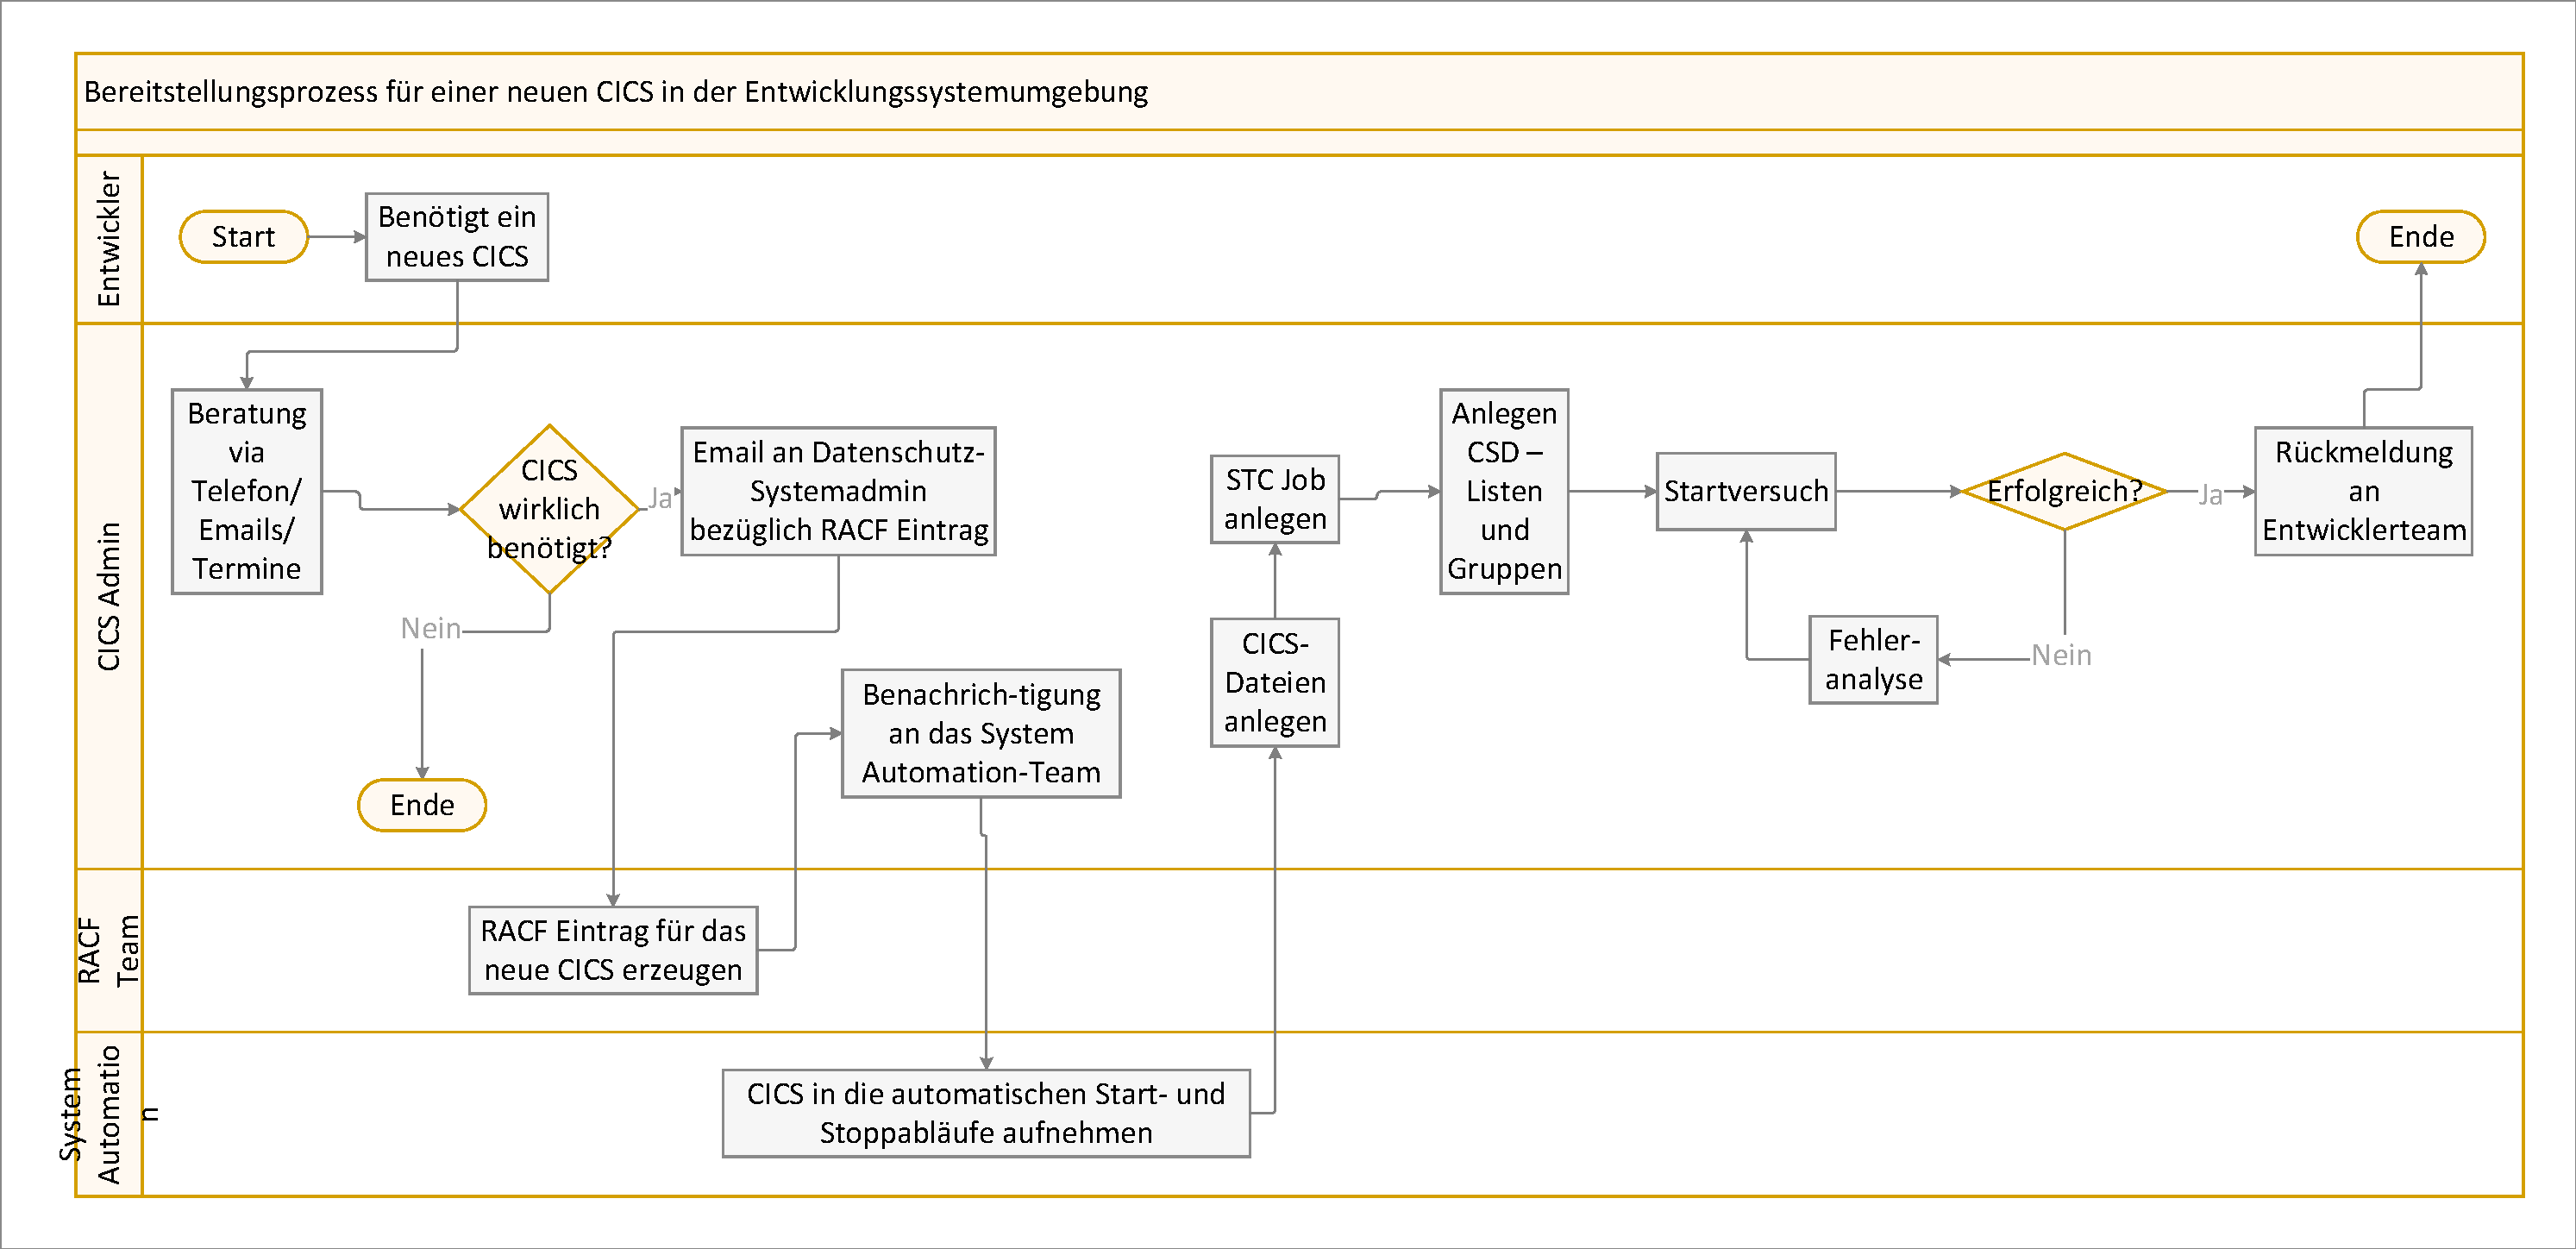
\includegraphics[width=\paperwidth,angle=90]{figures/swimlaneCICS.pdf}
\caption{Bereistellungsprozess einer CICS-Instanz}
\label{fig:aktcics}
\end{figure}

\begin{figure}[ht!]
\centering
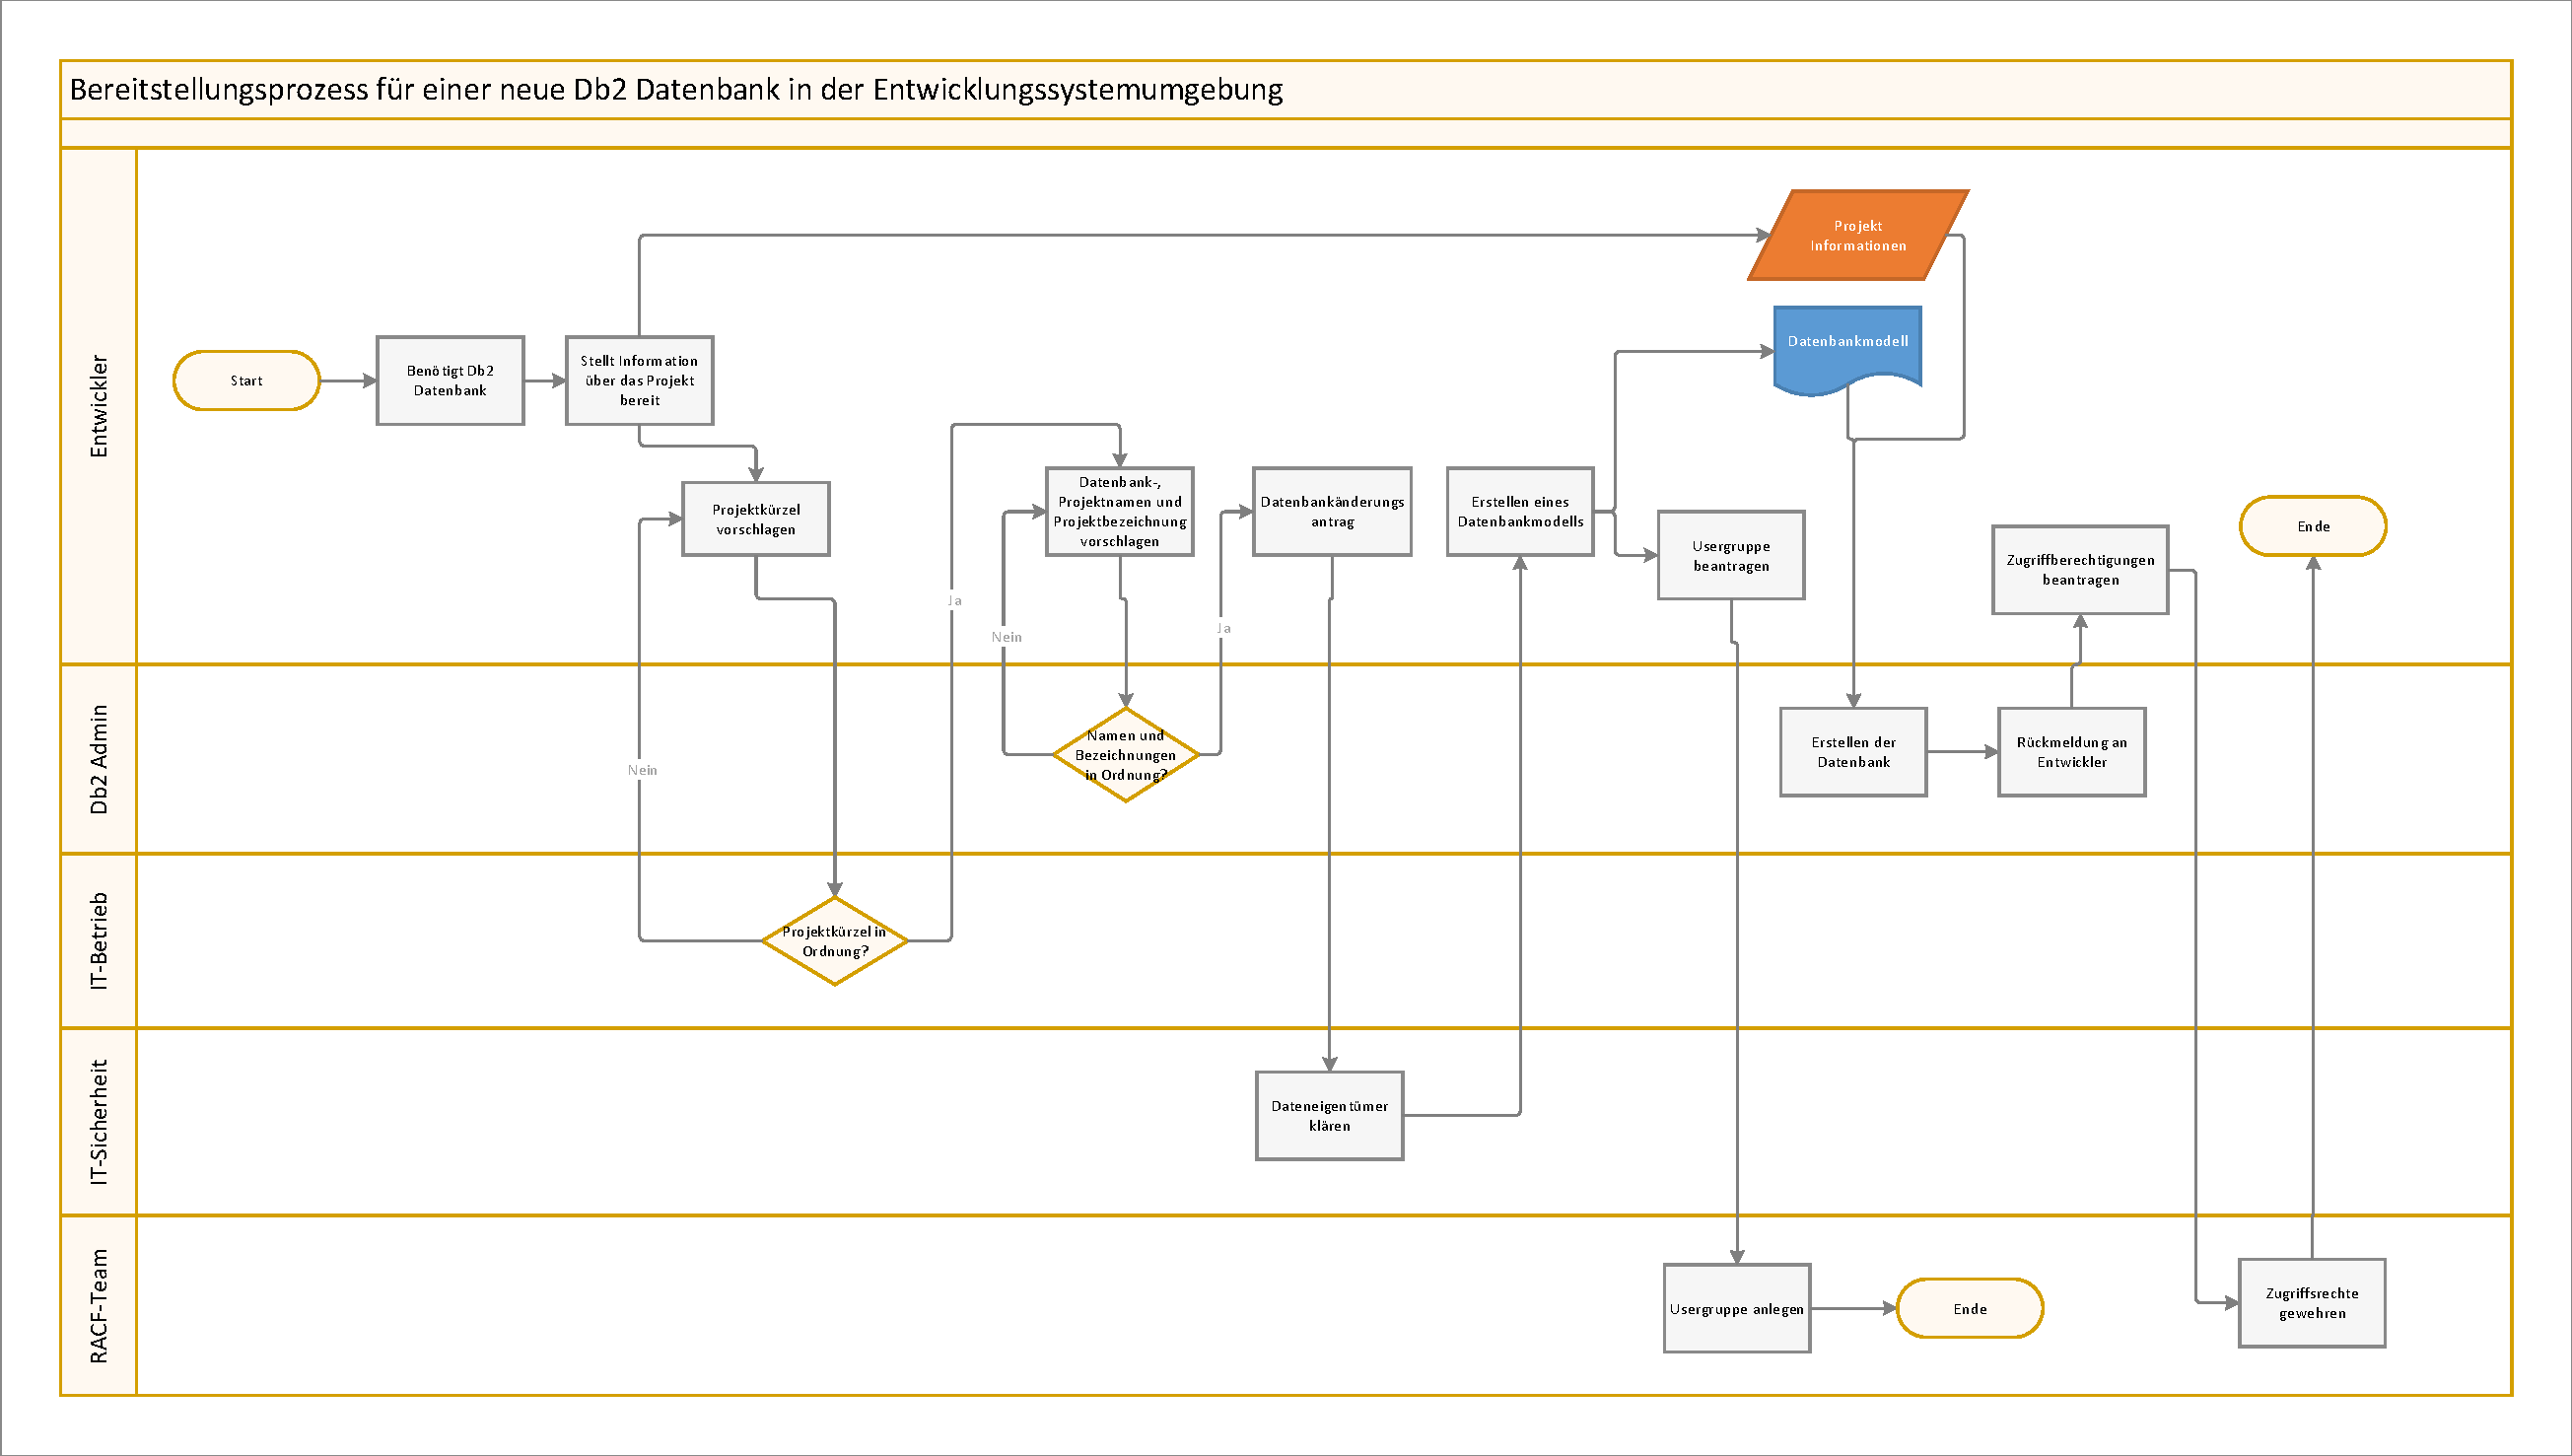
\includegraphics[width=\paperwidth,angle=90]{figures/swimlaneDb2.pdf}
\caption{Bereistellungsprozess einer Db2 Datenbank}
\label{fig:aktdb2}
\end{figure}

\begin{figure}[ht!]
\centering
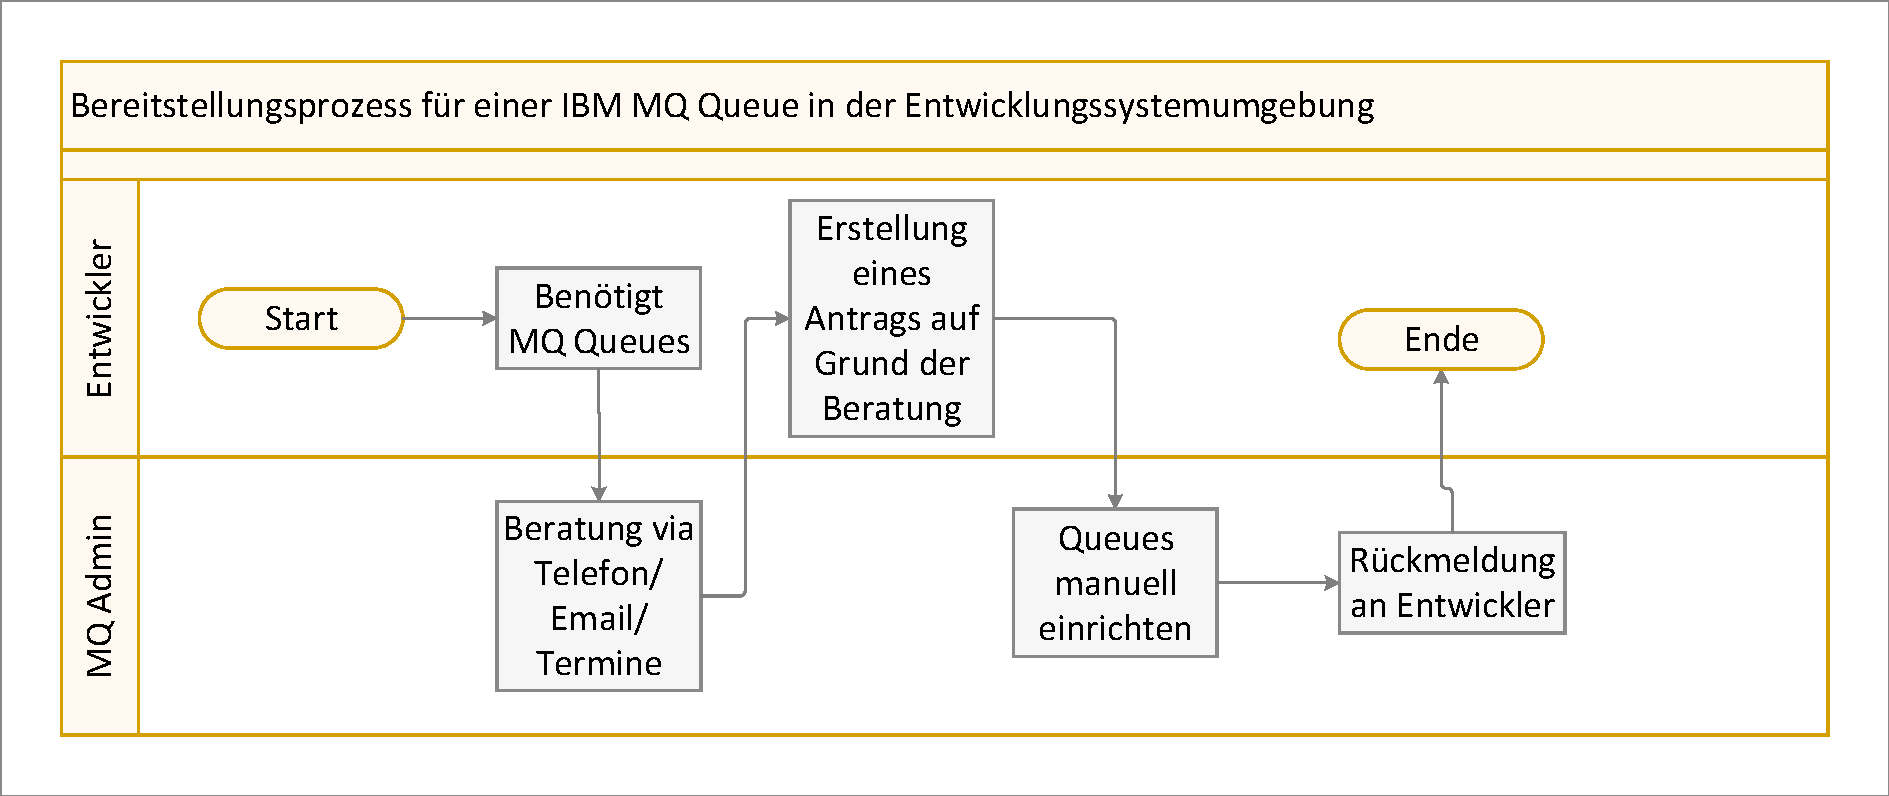
\includegraphics[width=\paperwidth,angle=90]{figures/swimlaneMQ.pdf}
\caption{Bereistellungsprozess einer IBM MQ Queue}
\label{fig:aktmq}
\end{figure}

Wie in den drei Diagrammen, Abbildungen \ref{fig:aktcics}, \ref{fig:aktdb2} und \ref{fig:aktmq}, zu erkennen ist, ist der aktuelle Bereitstellungsprozess noch mit vielen manuellen Schritten verbunden.
Außerdem ist der Hauptaufwand in den Administratorenteams angesiedelt.
Das Entwicklerteam ist der Initiator des Ablaufs.
Folglich kümmert es sich um Formulare und die erste Kontaktaufnahme zum Administratorenteam.
Bei dem Bereitstellungsprozess einer Db2 Datenbank muss es außerdem Projektinformationen, unter anderem Daten der Voruntersuchung, bereitstellen.
Hinzu kommt das Erstellen eines Datenbankmodells.
Hierfür wird Datenbankwissen benötigt, hierzu wird gegenfalls die Unterstützung eines Administrator benötigt.

Zusätzlich zu den vielen manuellen Schritten sind die vielen Absprachen zwischen mehreren Abteilungen zu nennen.
Steht ein beteiligtes Team nicht zu Verfügung, kommt es zu Verzögerungen, das Team muss warten, der komplette Zeitplan kann sich dadurch nach hinten verschieben.
Der Prozess für die Bereitstellung einer CICS-Instanz, mit einer Db2 Datenbank und IBM MQ Queues dauert in der Summe circa sechs Arbeitstage.
Es setzt sich aus der Dauer der Einzelprozesse zusammen, für jedes Subsystem wird mit circa zwei Arbeitstagen gerechnet.
Diese Einschätzung beruht auf den Annahmen, dass zum einen jedes beteiligte Team nur diese Aufgabe zu erledigen hat und zum anderen jeweils ein Tag für die Beratung durch das jeweilige Administratorenteam veranschlagt wird.
Natürlich ist ein parallelisierter Ablauf der einzelnen Teilprozesse möglich, so kann die Gesamtdauer im besten Fall auf circa zwei bis drei Arbeitstage verkürzt werden.

Ein weiterer Punkt ist, dass die Kommunikation beziehungsweise der Initiator für den Start des gesamten Prozesses meist per Zuruf stattfindet.
So existiert für die erste Kontaktaufnahme kein Formular, keine Automation oder ähnliches.
Zur Kommunikation wird auf E-Mail, Telefon oder mittels Terminen zurückgegriffen.

\section{CICS Bereitstellungsablauf}

\paragraph{Voraussetzungen}\label{subsec:voraus} ~\\
Bei der DATEV e.G. kümmert sich ein Team, die \glqq CICS Administration\grqq{} um das Erstellen einer CICS-Instanz, starten dieser Instanz und ist generell für alles rund um die Administration des CICS Transactions Servers zuständig.
Der Fokus dieser Arbeit liegt auf dem Erstellen (\glqq Provisionieren\grqq{}) einer CICS-Instanz. Es werden nur die dafür notwendigen Voraussetzungen dargelegt.
Außerdem liegt der Fokus auf Entwicklungs-CICS-Systemen, auf der sog. Entwicklungs-Stage, nicht auf den produktiven CICS-Systemen der DATEV e.G.. 
Aus diesem Grund werden nur Schritte, die für ein solches Testsystem benötigt werden, dargestellt.
Eine weitere Rahmenbedingung besteht darin, dass nur die Arbeitsschritte, die mit z/OSMF\footnote{Beschreibung in Absatz \ref{sec:zosmf}} automatisiert werden, erläutert werden.

\paragraph{Einrichtung CICS Instanz}\label{subsec:createCICS}~\\
Die in diesem Absatz benötigten Informationen stammen aus Gesprächen mit Mitarbeiter 2 aus der Abteilung, die für die CICS Administration zuständig ist.
Um eine lauffähige CICS Instanz den Voraussetzungen aus dem Absatz \ref{subsec:voraus} entsprechend einzurichten, sind mehrere Schritte notwendig.
Diese werden im Folgenden beschrieben.

\subparagraph{CICS spezifische Dateien}\label{sssec:speziDat} ~\\
Zunächst müssen CICS spezifische Dateien im z/OS angelegt werden.
Im Fall des dieser Arbeit zugrunde liegenden Beispiels handelt es sich um siebzehn verschiedene VSAM\footnote{Virtual Storage Access Method, spezielle Dateiart, die schnelle I/O-Zugriffe ermöglicht.\cite{Lovelace.2013}} Dateien.
Diese Dateien benötigt die CICS Instanz um zum Beispiel Systemfehler zu protokollieren oder den Debugger aktivieren zu können.

\subparagraph{CSD} ~\\
In der Datei \glqq CICS System Definition\grqq, kurz CSD, muss jede Ressource, die dem System zur Verfügung stehen soll, definiert werden.
Eine CSD Datei kann für mehrere CICS Instanzen verwendet werden und besteht aus mehreren Einträgen.
Ein Eintrag besteht aus einer Gruppe und einer Liste.
Die Gruppe ist hierbei die Definition einer Systemressource und muss manuell angelegt werden.
Bei der Liste handelt es sich um das System, welches diese Ressource benötigt.
Dort ist unter anderem für jede CICS Instanz hinterlegt, zu welchem Db2 Datenbanksystem und welchem IBM MQ Messagingsystem sich diese Instanz verbinden soll.

\subparagraph{STC Job} ~\\
Bei einem Started Task Control-Job, kurz STC Job, handelt es sich um einen Batch Job, der mit Hilfe des \glqq START\grqq-Konsolenkommandos innerhalb von z/OS gestartet werden kann.
Dieser Batch Job wird deshalb auch als Started Task bezeichnet.\cite{Cassier.2007}
Bei der DATEV eG existiert für jede Instanz eines Subsystems ein solcher Job, so also auch für CICS.
In diesem werden zunächst einige zur Laufzeit benötigten Bibliotheken und Dateien eingebunden, unter anderem die CICS spezifischen Dateien\footnote{Beschreibung in Absatz \ref{sssec:speziDat}}.
Außerdem werden hier die SIT \footnote{CICS system initialization table} Parameter definiert.
Zunächst wird festgelegt welche Standard SIT verwendet werden soll.
Anschließend können diese Standardwerte überschrieben werden.
Zu diesen Parametern zählen unter anderem der eindeutige Name der CICS-Instanz, der Speicherort der dazugehörenden CSD und die Information, ob eine Verbindung zu einem Db2 Datenbanksystem hergestellt werden soll.

\paragraph{Entfernung CICS Instanz} ~\\
Um eine CICS Instanz zu entfernen muss diese zunächst gestoppt werden.
Dies ist über das \glqq STOP\grqq-Konsolenkommando von z/OS möglich.
Schließlich müssen alle im Absatz \ref{subsec:createCICS} beschriebenen Schritte rückgängig gemacht werden.
Also müssen die für diese Instanz spezifischen Dateien, die Einträge für die CICS-Instanz aus der CSD Datei und schließlich auch der STC Job gelöscht werden.
 
